\documentclass[twocolumn,english]{IEEEtran}
\usepackage[T1]{fontenc}
\usepackage{babel}
\usepackage{amsthm}
\usepackage{amsmath}
\usepackage{graphicx}
\usepackage[unicode=true,
bookmarks=true,bookmarksnumbered=true,bookmarksopen=true,bookmarksopenlevel=1,
breaklinks=false,pdfborder={0 0 0},backref=false,colorlinks=false]
{hyperref}
\usepackage{bm}
\usepackage{amsmath}
\usepackage{amssymb}
\usepackage{natbib}
\usepackage{siunitx}
\usepackage{array}
\usepackage{calc}
\newcolumntype{W}{>{\centering\arraybackslash}m{25mm}}
\newcolumntype{L}{>{\centering\arraybackslash}m{15mm}}
\frenchspacing %Keeps spacing between sentences constant?

\hypersetup{
pdftitle=  {Capacitors},
pdfauthor= {Zack Garza},
pdfpagelayout=OneColumn, pdfnewwindow=true, pdfstartview=XYZ, plainpages=false}

\makeatletter


%%%%%%%%%%%%%%%%%%%%%%%%%%%%%% Textclass specific LaTeX commands.
% protect \markboth against an old bug reintroduced in babel >= 3.8g
\let\oldforeign@language\foreign@language
\DeclareRobustCommand{\foreign@language}[1]{%
  \lowercase{\oldforeign@language{#1}}}
\theoremstyle{plain}
\newtheorem{thm}{\protect\theoremname}
\theoremstyle{plain}
\newtheorem{lem}[thm]{\protect\lemmaname}

%%%%%%%%%%%%%%%%%%%%%%%%%%%%%% User specified LaTeX commands.
% for subfigures/subtables
\ifCLASSOPTIONcompsoc
\usepackage[caption=false,font=normalsize,labelfont=sf,textfont=sf]{subfig}
\else
\usepackage[caption=false,font=footnotesize]{subfig}
\fi

\makeatother
\providecommand{\lemmaname}{Lemma}
\providecommand{\theoremname}{Theorem}
\sisetup{detect-weight=true, detect-family=true}
\setcounter{topnumber}{2}
\setcounter{bottomnumber}{2}
\setcounter{totalnumber}{4}
\renewcommand{\topfraction}{0.85}
\renewcommand{\bottomfraction}{0.85}
\renewcommand{\textfraction}{0.15}
\renewcommand{\floatpagefraction}{0.7}
\usepackage{float}
\begin{document}

\title{Capacitors}


\author{Zack Garza}


\IEEEspecialpapernotice
{Physics 210L \\
Effective Date of Report: March 6, 2014}


\markboth{Capacitors}{Zack Garza}
\maketitle

\tableofcontents

\section{Introduction}
\IEEEPARstart{T}{he} purpose of this experiment is to verify some of the relationships involving capacitance and, in the process, learn more about capacitors. Since they are our first major circuit element,you will also be developing your ability to work with circuits. Specifically, you will:
\begin{enumerate}
\item Use an LCR to measure $C_m$ for this capacitor as a function of $d$ and compare the results to the theoretical results obtained from Gauss' Law.
\item Ti measure the dielectric constant of a material and observe the effect of dielectrics on capacitance.
\item To verify the relationships for equivalent capacitance for both series and parallel capacitors using the LCR meter.
\end{enumerate}

\section{Theory}
Using your text, show complete derivations and/or explanations for each of the following important relationships: \\

\noindent\textbf{For a Parallel Plate Capacitor}

\begin{enumerate}
\item $C={\epsilon}_0 A/d$

  Capacitance is defined as the ratio of the magnitude of the charge on a conductor divided by the magnitude of the potential difference between them. As such, the capacitance can be written
  \begin{equation}\label{eq:capacitance}
  C=Q/\Delta V.
  \end{equation}
  In the case of parallel-plate capacitors with equal area $A$ separated by a distance $d$, both plates carry an equal charge of magnitude $Q$. Since a higher surface area results provides more space for charge to be stored, it is expected that $C\propto A$.

  Taking the plate separation $d$ to be much smaller than $A$, the electric field between the plates can be approximated as uniform everywhere between the plates and zero elsewhere. If a power source supplies a constant potential, from the expression $\Delta V = Ed$, an increase in the distance would tend to increase the potential difference, and since $C=Q/\Delta V$, $C\propto 1/d$.

  It can be shown that the electric field of an infinite plate is $E=\sigma / \epsilon_0$. If each plate has a surface charge density of $\sigma = Q/A$, then
  \begin{equation*}
  E = \frac{\sigma}{\epsilon_0 A}.
  \end{equation*}

  Which when substituted into $\Delta V = Ed$ yields
  \begin{equation}\label{eq:deltav}
  \Delta V = \frac{dQ}{\epsilon_0 A}.
  \end{equation}

  Substituting equation~\ref{eq:deltav} into equation~\ref{eq:capacitance} then gives an expression for capacitance in terms of its surface area $A$ and plate separation $d$.~\cite{serway2013physics}
  \begin{align}\label{eq:finalcapeq}
  C &= \frac{Q}{\Delta V} = \frac{Q}{Qd/ \epsilon_0 A} \Rightarrow \notag \\
  C &= \frac{\epsilon_0 A}{d}
  \end{align}


\item $C=kC_0=k{\epsilon}_0 A/d$

When a dielectric composed of polar molecules is placed in a uniform electric field, the randomly oriented dipoles will tend to align with the electric field - that is, the positive portions will be pulled toward the negative plate, and vice versa. This produces a net dipole moment and hence a net electric field that is directed opposite to the electric field between the plates. From $\Delta V = Ed$, decreasing $E$ will decrease $\Delta V$, so it can be said that the presence of a dielectric lowers $\Delta V$ by a factor $\kappa$. That is,
\begin{equation}\label{eq:kappa1}
  \Delta V = \frac{\Delta V_0}{\kappa}.
\end{equation}


If the capacitor is an isolated system -- that is, the amount of charge on each plate remains constant -- then examining the expression for capacitance in equation~\ref{eq:finalcapeq} shows that a change in $\Delta V$ necessarily implies a change in $C$. Substituting equation~\ref{eq:kappa1} into equation~\ref{eq:finalcapeq} yields
\begin{gather}\label{eq:kappa}
  C = \frac{Q}{\Delta V} = \frac{Q}{\Delta V_0 / \kappa} = \kappa \left(\frac{Q}{\Delta V_0}\right) \Rightarrow \notag \\
  C = \kappa C_0 = \frac{\kappa \epsilon_0 A}{d}
\end{gather}
\end{enumerate}

\noindent \hrulefill

\noindent \textbf{Adding Capacitors in Parallel}

\noindent$C_{\text{eq}}=C_1+C_2+C_3...+C_n$

  \begin{figure}[h!]
  \begin{centering}
  \begin{center}
  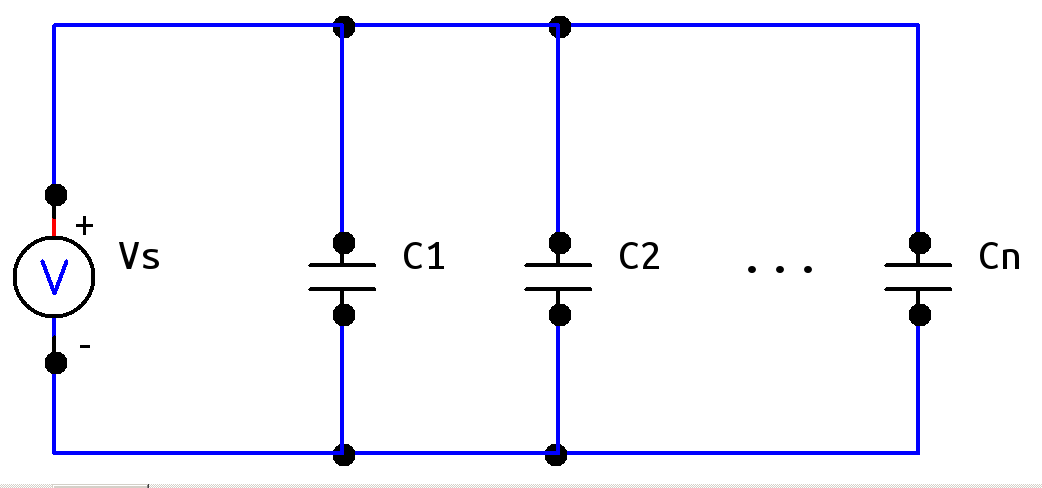
\includegraphics[width=\linewidth]{./Pictures/parallelc.png}
  \label{fig:parallel_diagram}
  \caption{$n$ Capacitors Wired in Parallel}
  \end{center}
  \par\end{centering}
  \end{figure}

  Consider a system of $n$ capacitors wired in parallel, as shown in Figure~\ref{fig:parallel_diagram}.

  To simplify this system, an expression for an equivalent capacitance $C_{eq}$ can be found that behaves exactly as the collection of $n$ capacitors.

  At steady state, each capacitor accrues a maximum charge $Q_n$. The total charge of the system is then
  \begin{equation}\label{eq:qdots}
  Q_{tot} = Q_1 + Q_2 + \dots Q_n = \sum_{i=1}^{n} Q_i
  \end{equation}

  Rearranging the expression for capacitance in equation~\ref{eq:capacitance} yields $Q=C\Delta V$, and substituting this into equation~\ref{eq:qdots} yields
  \begin{equation*}
  \frac{C_{eq}}{\Delta V_{tot}} = \sum_{i=1}^{n} \frac{C_n}{\Delta V_n}
  \end{equation*}

  Since the wires in such a circuit are modeled as ideal conductors, the potential along any given wire must be everywhere the same, and the potential difference between the plates of each capacitor is equal to the potential difference across the source. Thus, $\Delta V_{tot} = \Delta V_n$, and factoring this term out of both sides of the equation shows that
  \begin{equation}
  C_{eq} = \sum_{i=1}^{n} C_n,
  \end{equation}
  or that the equivalent capacitance of parallel capacitors is simply the sum of the individual capacitance values.

  \noindent \hrulefill

\noindent \textbf{Adding Capacitors in Series}

\noindent$1/C_{\text{eq}}=1/C_1 + 1/C_2\cdots+1/C_n$

  \begin{figure}[h!]
  \begin{centering}
  \begin{center}
  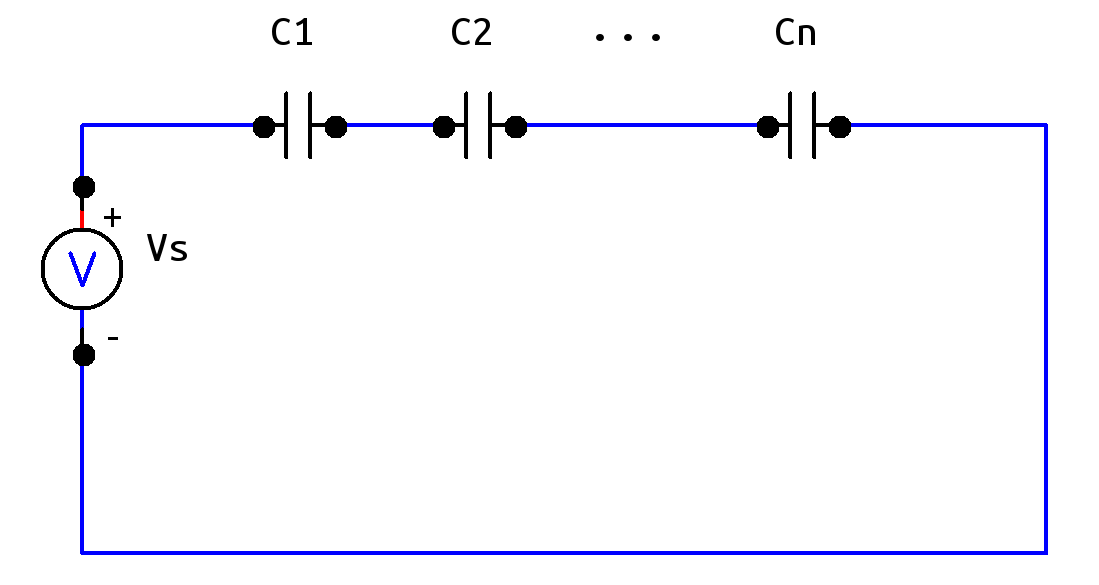
\includegraphics[width=\linewidth]{./Pictures/seriesc.png}
  \label{fig:series_diagram}
  \caption{$n$ Capacitors Wired in Series}
  \end{center}
  \par\end{centering}
  \end{figure}

  Similarly, now consider a system of $n$ capacitors wired in series as shown in figure ~\ref{fig:series_diagram}. To find an equivalent capacitance $C_{eq}$, note that since either end of the system is connected to a voltage source, the sum of the voltages through each resistor will be equal to the potential difference across the source, such that

  \begin{equation}\label{eq:qseriesdots}
  \Delta V_{source} = \Delta V_1 + \Delta V_2 + \dots \Delta V_n = \sum_{i=1}^{n} \Delta V_i
  \end{equation}

  Rearranging equation~\ref{eq:capacitance} shows that $\Delta V=Q/C$, and substituting this into equation~\ref{eq:qseriesdots} yields
  \begin{equation*}
  \frac{Q_{tot}}{C_{eq}} = \sum_{i=1}^{n} \frac{Q_n}{C_n}
  \end{equation*}

  A capacitor is modeled by the movement of electrons from one plate to another, and so the charge on any given plate will induce an equal and opposite charge on any other plate that is connected by a conductor. It can be shown that $Q$ is equal for every capacitor in series, and that an equivalent capacitor would also have a charge $Q$. Setting $Q_{tot} = {Q_n}$ and factoring out the constant term shows that
  \begin{equation}
  \frac{1}{C_{eq}} = \sum_{i=1}^{n} \frac{1}{C_n},
  \end{equation}
  or that the inverse of the equivalent capacitance of capacitors in a series can be expressed as the sum of the inverse of each individual capacitance.

\section{Methodology}

\subsection*{Part 1}
Connect the LCR meter to the sliding capacitor and measure $d$ and $c$ for up to 5 cm of separation. Collect at least ten data points. Also measure the area of the plates.
\subsection*{Part 2}
Measure $C_0$ for the demountable capacitor with the spacers in place. Insert the mica dielectric and measure $C_k$.
\subsection*{Part 3}
Measure $C$ for the two demountable capacitors separately. Connect them in series and parallel and measure $C_eq$ for each arrangement with the spacers in place.
\subsection*{Part 4}
Given three capacitor substitution boxes, wire the circuit shown below. The value of the two capacitors must be different. Set the signal generator to generate a 1000 Hz sine wave. Set the voltage of the generator to approximately 4 V as measured by a multi-meter, using the AC setting. Record the capacitance of each capacitor, and measure the voltage across capacitor $C_3$.

\begin{figure}[h!]
\begin{centering}
  \begin{center}
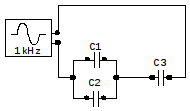
\includegraphics[keepaspectratio=true]{./Pictures/diagram1.png}
\label{fig:circuit_diagram1}
\caption{Circuit Diagram for Capacitor Substitution Box}
\end{center}
\par\end{centering}
\end{figure}



\section{Data}
  \subsection*{\textbf{Part 1}}
  \begin{centering}
  \begin{table}[!htbp]\label{tb:data}
    \caption{Capacitance as Distance Between Plates is Increased}
    \centering{}
    \begin{tabular}{ |c|c|c|}
    \hline
    \textbf{Trial} & \textbf{$d$ (cm)} & \textbf{$C$ (pF)} \\ \hline
    1   & .30  & 108.8  \\ \hline
    2   & .40  & 84.9  \\ \hline
    3   & .50  & 69.7  \\ \hline
    4   & .60  & 58.7  \\ \hline
    5   & .70  & 52.2  \\ \hline
    6   & .80  & 47.9  \\ \hline
    7   & .90  & 42.9  \\ \hline
    8   & 1.0  & 39.3  \\ \hline
    9   & 1.5  & 29.3  \\ \hline
    10  & 2.0  & 24.1  \\ \hline
    11  & 2.5  & 20.9  \\ \hline
    12  & 3.0  & 18.8  \\ \hline
    13  & 3.5  & 17.3  \\ \hline
    14  & 4.0  & 16.0  \\ \hline
    15  & 4.5  & 15.2  \\ \hline
    16  & 5.0  & 14.4  \\ \hline





    \end{tabular}
  \end{table}
  \end{centering}
  \begin{align*}
  \text{Diameter of Cylindrical Plate: \underline{200.5 mm} }
  \end{align*}
  \subsection*{\textbf{Part 2}}
  \begin{align*}
  &C_0: \text{:\underline{.415 nF}} &C: \text{\underline{.337 nF}}
  \end{align*}
  \subsection*{\textbf{Part 3}}
  \begin{align*}
  &C_1: \text{\underline{.433 nF}} &C_2: \text{\underline{.415 nF}} \\
  &C_p: \text{\underline{.846 nF}} &C_s: \text{\underline{.211 nF}}
  \end{align*}
  \subsection*{\textbf{Part 4}}
  \begin{align*}
  &C_1:\text{\underline{25.5 $\mu$F}} & &C_2:\text{\underline{50.8 $\mu$F}} & &C_3:\text{\underline{76.0 $\mu$F}}
  \end{align*}\\
  \begin{center}
  Measured Values
  \end{center}
  \begin{align*}
  &V_3: \text{\underline{1.978 V}} &V_{\text{Battery}}: \text{\underline{3.948 V}}
  \end{align*}


\section{Analysis}
  \subsection*{\textbf{Part 1}}
  \textit{Graph $C$ vs. $1/d$ (explaining why), and evaluate the slope. Calculate $\epsilon_0$ from the slope along with its estimated uncertainty, taken from the uncertainty in $d$, $A$, and the uncertainty of the slope in your curve fit. Then compare it to the accepted values by calculating a percent error. Show units and all work.}

  \begin{figure}[h!]
  \begin{centering}
  \begin{center}
  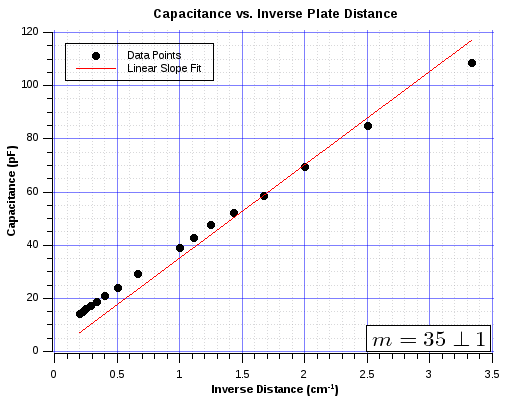
\includegraphics[width=\linewidth]{./Pictures/graph1.png}
  \label{fig:graph1}
  \caption{Plot of Table~\ref{tb:data} Data}
  \end{center}
  \par\end{centering}
  \end{figure}

  From equation~\ref{eq:capacitance}, taking $1/d$ as the independent variable, the slope $m$ must be equal to $\epsilon_0 A$, and so $\epsilon_0 = m/A$. Unit conversions are needed, as the theoretical value of $\epsilon_0$ is in terms of $F/m$. Since the plates are circular, the area is $\pi r^2$, and using the $1/2$ value of the measured diameter yields $A=.03157 m^2$.
  \begin{equation*}
   \epsilon_0 = \frac{m}{A} = \frac{ (35 pF\cdot cm) (\frac{1 m}{100 cm})(\frac{1 F}{10^{12} pF})}{.03157 m^2} = 1.108 \times 10^{-11} \frac{F}{m}
  \end{equation*}
  Taking the theoretical value of $\epsilon_0$ as $8.854\times 10^{-12} F/m$, the percent error is
  \begin{align*}
   \left(\frac{1.108\times 10^{-11} F/m - 8.854\times 10^{-12}F/m}{8.854\times 10^{-12}F/m}\right)\times 100\% \\
   = 25.14\%
  \end{align*}

  In order to calculate the total uncertainty, several values are needed. Expressing the equation as $\epsilon_0 = m/A$ and substituting rewriting $A$ in terms of the measured diameter $d$ yields
  \begin{align*}
   \epsilon_0= \frac{4m}{\pi d^2}
  \end{align*}
  which shows that the independent variables are both $m$ and $d$. Since the squares of partial derivatives of both functions are needed, they are computed and evaluated as follows.
  \begin{align*}
   \left(\frac{\partial \epsilon_0}{\partial m}\right)^2 =& \left(\frac{4}{\pi d^2}\right)^2 \\
   =& \left(\frac{4}{\pi (.2005 m)^2}\right)^2 \\
   =& (31.67)^2 =1003 \\
   \left(\frac{\partial \epsilon_0}{\partial d}\right)^2 =& \left(\frac{-8m}{\pi d^3}\right)^2 \\
   =& \left(\frac{-8\cdot 3.5\times 10^{-13} F\cdot m}{\pi (.2005 m)^3}\right)^2
   = 1.22 \times 10^{-18}
  \end{align*}
  The uncertainties are also needed, so $\delta_m$ is taken to be the uncertainty from the linear fit. The units are converted beforehand to ensure that the total calculated uncertainty is in terms of $F/m$.
  \begin{align*}
   \delta_m = 1 pF\cdot cm \times (\frac{1 F}{10^{12} pF}) \times (\frac{1 m}{100 cm}) = 1 \times 10^{-13} F\cdot m
  \end{align*}
  The uncertainty in the diameter $\delta_d$ is taken to be the resolution of the meter stick used, which was marked to the nearest millimeter. Converting this to meters yields
  \begin{align*}
   \delta_d = .5 mm \times (\frac{1 m}{1000 mm}) = 5\times 10^{-4} m
  \end{align*}
  Taking the equation for error propagation and substituting in the previously derived values gives the total uncertainty $\delta_{\epsilon}$.
  \begin{align*}
   \delta_{\epsilon} &= \sqrt{(\frac{\partial \epsilon_0}{\partial m})^2(\delta_m)^2 + (\frac{\partial \epsilon_0}{\partial d})^2(\delta_d)^2} \\
   &= \sqrt{(1003)(1\times 10^{-14})^2 + (1.22 \times 10^{-18})(5\times 10^{-4})^2} \\
   &= 6.36 \times 10^{-13} F/m
  \end{align*}


  \subsection*{\textbf{Part 2}}
  \textit{Calculate the dielectric constant for mica.}
  Dividing equation~\ref{eq:finalcapeq} by equation~\ref{eq:kappa} yields
  \begin{equation}
   \frac{C_{\kappa}}{C_0} = \kappa
  \end{equation}
  Substituting in the measured values yields
  \begin{equation*}
   \kappa = \frac{C_{\kappa}}{C_0} = \frac{.337 nF}{.415 nF} = .812
  \end{equation*}


  \subsection*{\textbf{Part 3}}
  \textit{Calculate $C_{eq}$ for both the parallel and series capacitance and compare it with the measured values with \% error.}
  Using the equations from the Theory section for capacitors in parallel, the equivalent capacitance of $C_1$ and $C_2$
  \begin{align*}
   C_{eq} = C_1 + C_2 = .433 nF + .415 nF = .848 nF \\
   \text{\% Difference: } \frac{.848 nF - .846 nF}{.846 pF} \times 100\% = 0.2\%
  \end{align*}
  For the capacitors in series,
  \begin{align*}
  \frac{1}{C_{eq}} 	=& \frac{1}{C_1} + \frac{1}{C_2} \\
  		     	=& \frac{1}{.433 nF} + \frac{1}{.415 nF} \\
  		     	=& (2.309) + (2.410) \\
  \Rightarrow C_{eq} 	=& .212 nF \\
  \text{\% Difference} =& \frac{.211 nF - .212 nF}{.212 nF} = -.5\%
  \end{align*}


  \subsection*{\textbf{Part 4}}
  \textit{Calculate the theoretical values for $V_3$, the voltage across capacitor $C_3$, and compared it with the measured value with \% error.}
  The voltage across all three capacitors must equal the source voltage. Letting $C_{eq1}$ be the equivalent capacitance of the parallel capacitors $C_1$ and $C_2$ and $\Delta V_{eq1}$ be the voltage across the parallel connection, then
  \begin{align*}
   \Delta V_s = \Delta V_{eq1} + \Delta V_3 \\
  \end{align*}
  Rewriting the above expression, noting that $Q = C \Delta V$ and letting $Q_{eq1}$ be the total charge in the parallel branch shows that
  \begin{align*}
   \Delta V_s = \frac{Q_{eq1}}{C_{eq1}} + \Delta V_3
  \end{align*}
  Because the parallel branch is in series with $C_3$, the charge in $C_{eq1}$ must be equal to the charge on $C_3$
  \begin{align*}
   Q_{eq1} =& Q_3 = C_3 \Delta V_3 \Rightarrow \\
   \Delta V_s 	=& \frac{C_3 \Delta V_3}{C_{eq1}} + \Delta V_3 \\
		=& \Delta V_3 (\frac{C_3}{C_{eq1}} +1)
  \end{align*}
  Solving for $\Delta V_3$, noting that $C_{eq1} = C_1 + C_2$, and substituting in the known values yields the theoretical voltage over $C_3$
  \begin{align*}
   \Delta V_3 	=& \frac{\Delta V_s}{1 + (C_3 / C_{eq1})} \\
		=& \frac{3.948 V}{1 + (76.0 \mu F / (25.5 \mu F + 50.8 \mu F))} \\
		=& 1.977 V
  \end{align*}
  Calculating the percent difference:
  \begin{align*}
   \text{\% Difference: }\frac{1.978 V - 1.977 V }{1.977 V}\times 100\% = .05\%
  \end{align*}





\section{Results}
  \subsection*{\textbf{Part 1}}
  \begin{align*}
  \epsilon_0:& \,1.1 \times 10^{-11} \pm .06 \times 10^{-11} F/m \\
  \text{Percent Error:}& \,25.140\%
  \end{align*}
  \textit{Is the error in the result above mainly random or systematic? Explain.}
  The error in this value is largely systematic. The value $\epsilon_0$ represents the permittivity of a vacuum, while the space between the plates is realistically filled with various air molecules. It follows that these can form a very weak dielectric material, increasing the permittivity while simultaneously slightly skewing the measured capacitance values. It would be expected that these factors would tend to result in an increased value in calculated permittivity, which the results reflected.

  \subsection*{\textbf{Part 2}}
  \begin{align*}
  &\kappa: .812
  \end{align*}

  \subsection*{\textbf{Part 3: Calculated Capacitance Values}}
  \begin{align*}
  &\text{\underline{Parallel}}	&				&	&\text{\underline{Series}}&		& 			      &			\\
  &C_{\text{eq}}:	&\text .848 nF			&	&C_{\text{eq}}:&	&.212 nF&			\\
  &\text{\% Error:}	&.2\%				&	&\text{\% Error:}&	&-.5\%&			\\
  \end{align*}

  \subsection*{\textbf{Part 4}}
  \begin{align*}
  &\text{\underline{Measured Values}} & &\text{\underline{Theoretical Values}} & 	&\text{\underline{Percent Error}}\\
  &V_3: 1.978 V 	& 		&V_3: 1.977 V & 		& .05\%
  \end{align*}


\bibliographystyle{plain}
\bibliography{physbib}

\end{document}